%% ============================================================================
%% fig_2_6_lora_v1_pipeline.tex -- TikZ source of thesis Figure 11 (label
%% fig:lora_v1_pipeline, Ch.2).
%% Facts checked in 05-experimental/CLAM_TR_LoRA_v1_FIXED_v8_SHARDED.ipynb:
%%   Stage 0 one frozen-feature SpatialMultRetNet_bestHP fold checkpoint scores every
%%           patch, keeps topk(min(128, n)) indices + coordinates (cell 19);
%%   Stage 1 reads the selected patches from the .tiff slides at 20x (cells 21-22);
%%   Stage 2 LoRA r = 8, lora_alpha = 16, lora_dropout = 0.05, target qkv, jointly
%%           with a SpatialMultRetNet head; 10 epochs, patience 5, focal loss,
%%           label smoothing 0.1 (cells 11, 26, 28, 32);
%%   Stage 3 re-tiles with 224-px patches at 20x, slide in fold n encoded by the
%%           fold-n checkpoint (cell 34); 5,516,732 patches (cell 36 output);
%%   Stage 4 12 configurations x 5 folds, 50 epochs, default lr 1e-4 (cell 36).
%% Outcome line = thesis appendix app:lora_outcome (0.9529 < 0.9543: no clear gain).
%%
%% Layout (KTU thesis guide, section 5.1: figure text >= 10 pt): five stacked rows
%% (heading | stage box -> output chip), all text at
%% 10 pt (normalsize of the 10 pt standalone; headings 10 pt bold), no \scriptsize,
%% no \DeclareMathSizes (math sub/superscripts at the standard 7 pt script size).
%% Natural width 14.65 cm <= 0.95 \textwidth (14.71 cm), so it prints at scale >= 1.
%% ============================================================================
\documentclass[border=1pt]{standalone}
\usepackage[T1]{fontenc}
\usepackage{newtxtext,newtxmath}
\usepackage{amsmath}
\usepackage{tikz}
\usetikzlibrary{positioning,arrows.meta,calc}

\definecolor{ink}{RGB}{28,36,58}
\definecolor{stfill}{RGB}{228,236,247}
\definecolor{stline}{RGB}{58,86,132}
\definecolor{chfill}{RGB}{236,236,236}
\definecolor{chline}{RGB}{120,120,120}
\definecolor{fusfill}{RGB}{220,240,214}
\definecolor{fusline}{RGB}{52,122,52}

% configuration names: typewriter at 10 pt (as in the body text)
\newcommand{\cfg}[1]{{\texttt{#1}}}
% outcome line under the status bar: \showoutcometrue or \showoutcomefalse
% OFF in the thesis: the Fig. 11 caption defers the outcome to the appendix and Ch.2 says the LoRA
% subsection describes the pipeline only; the verdict (no clear gain) is stated in Ch.4 sec:sub5_lora and the appendix.
\newif\ifshowoutcome \showoutcomefalse
% box body: main text + detail paragraph (both 10 pt)
\newcommand{\body}[2]{#1\par\vspace{4.5pt}#2\par}

\begin{document}
\hyphenpenalty=10000 \exhyphenpenalty=10000
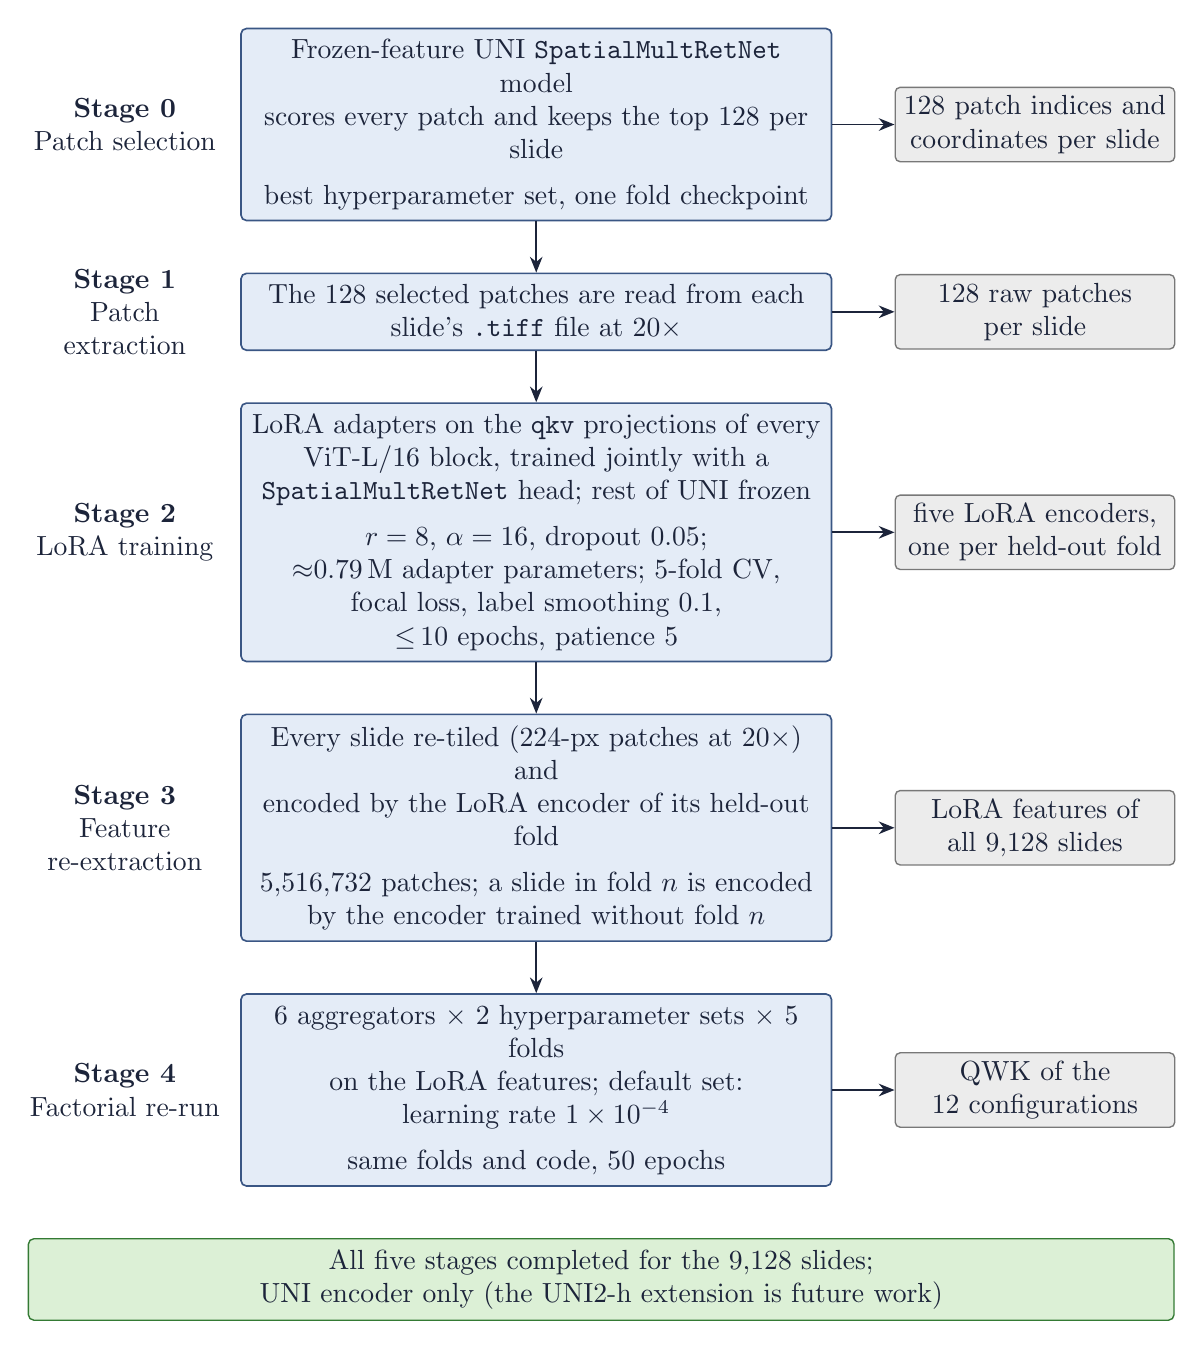
\begin{tikzpicture}[
  font=\normalsize, text=ink,
  >={Stealth[length=2.0mm,width=1.6mm]},
  stage/.style={draw=stline, fill=stfill, rounded corners=2pt, line width=0.6pt,
                align=flush center, inner xsep=4pt, inner ysep=4pt, text width=7.50cm-8pt,
                minimum width=7.50cm},
  chip/.style={draw=chline, fill=chfill, rounded corners=1.8pt, line width=0.5pt,
               align=flush center, inner xsep=3pt, inner ysep=3pt, text width=3.55cm-6pt,
               minimum width=3.55cm, anchor=west},
  hd/.style={align=flush center, text width=2.45cm, inner sep=0pt},
  ar/.style={->, line width=0.6pt, draw=ink},
  node distance=6.5mm
]

% column geometry (cm): heading column centre 1.225 (2.45 wide); stage boxes 2.70-10.20
% (centre 6.45); output chips 11.00-14.55; status bar 0-14.55.
\coordinate (hx) at (1.225,0);
\coordinate (cx) at (11.00,0);
\coordinate (mx) at (7.275,0);

% ------------------------------------------------------------------ stage boxes
\node[stage, anchor=north] (s0) at (6.45,0)
  {\body{Frozen-feature UNI \cfg{SpatialMultRetNet} model\\ scores every patch and keeps the top 128 per slide}
         {best hyperparameter set, one fold checkpoint}};
\node[stage, below=of s0] (s1)
  {The 128 selected patches are read from each\\ slide's \texttt{.tiff} file at $20\times$};
\node[stage, below=of s1] (s2)
  {\body{LoRA adapters on the \texttt{qkv} projections of every\\ \mbox{ViT-L/16} block, trained jointly with a\\ \cfg{SpatialMultRetNet} head; rest of UNI frozen}
         {$r=8$, $\alpha=16$, dropout 0.05;\\ $\approx$0.79\,M adapter parameters; 5-fold CV,\\ focal loss, label smoothing 0.1,\\ $\leq$\,10~epochs, patience~5}};
\node[stage, below=of s2] (s3)
  {\body{Every slide re-tiled (224-px patches at $20\times$) and\\ encoded by the LoRA encoder of its held-out fold}
         {5,516,732 patches; a slide in fold $n$ is encoded\\ by the encoder trained without fold $n$}};
\node[stage, below=of s3] (s4)
  {\body{6 aggregators $\times$ 2 hyperparameter sets $\times$ 5 folds\\ on the LoRA features; default set:\\ learning rate $1\times10^{-4}$}
         {same folds and code, 50 epochs}};

\foreach \u/\v in {s0/s1, s1/s2, s2/s3, s3/s4} \draw[ar] (\u.south) -- (\v.north);

% ------------------------------------------------------------------ headings (left of each stage)
\node[hd] at (hx |- s0.center) {\textbf{Stage 0}\\ Patch selection};
\node[hd] at (hx |- s1.center) {\textbf{Stage 1}\\ Patch extraction};
\node[hd] at (hx |- s2.center) {\textbf{Stage 2}\\ LoRA training};
\node[hd] at (hx |- s3.center) {\textbf{Stage 3}\\ Feature re-extraction};
\node[hd] at (hx |- s4.center) {\textbf{Stage 4}\\ Factorial re-run};

% ------------------------------------------------------------------ outputs (right of each stage)
\node[chip] (c0) at (cx |- s0.east) {128 patch indices and\\ coordinates per slide};
\node[chip] (c1) at (cx |- s1.east) {128 raw patches\\ per slide};
\node[chip] (c2) at (cx |- s2.east) {five LoRA encoders,\\ one per held-out fold};
\node[chip] (c3) at (cx |- s3.east) {LoRA features of\\ all 9,128 slides};
\node[chip] (c4) at (cx |- s4.east) {QWK of the\\ 12 configurations};
\foreach \u/\v in {s0/c0, s1/c1, s2/c2, s3/c3, s4/c4} \draw[ar] (\u.east) -- (\v.west);

% ------------------------------------------------------------------ status and outcome
\node[draw=fusline, fill=fusfill, line width=0.5pt, rounded corners=2pt, align=flush center,
      minimum width=14.55cm, text width=14.55cm-10pt, inner xsep=5pt, inner ysep=4pt,
      anchor=north] (st) at (mx |- s4.south) [yshift=-6.5mm]
  {All five stages completed for the 9,128 slides;\\ UNI encoder only (the UNI2-h extension is future work)};
\ifshowoutcome
\node[anchor=north, align=flush center, text width=14.55cm] at ($(st.south)+(0,-1.5mm)$)
  {\textbf{Outcome:} best LoRA-UNI configuration 0.9529 QWK, below the best frozen UNI configuration (0.9543): no clear gain};
\fi

\end{tikzpicture}
\end{document}
